% This file was created with tikzplotlib v0.10.1.
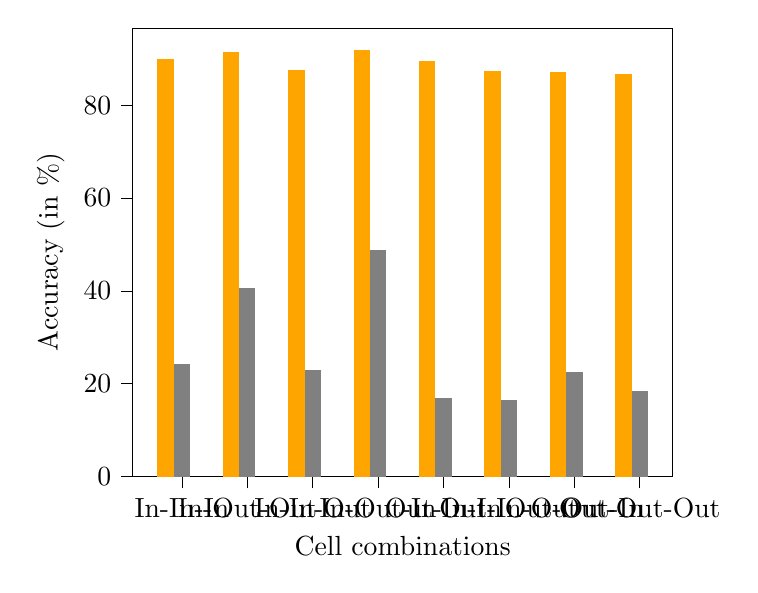
\begin{tikzpicture}

\definecolor{darkgray176}{RGB}{176,176,176}
\definecolor{gray}{RGB}{128,128,128}
\definecolor{lightgray204}{RGB}{204,204,204}
\definecolor{orange}{RGB}{255,165,0}

\begin{axis}[
legend cell align={left},
legend style={fill opacity=0.8, draw opacity=1, text opacity=1, draw=lightgray204},
tick align=outside,
tick pos=left,
x grid style={darkgray176},
xlabel={Cell combinations},
xmin=-0.75, xmax=7.5,
xtick style={color=black},
xtick={0,1,2,3,4,5,6,7},
xticklabels={
  In-In-In,
  In-Out-Out,
  In-In-Out,
  In-Out-In,
  Out-In-In,
  Out-In-Out,
  Out-Out-In,
  Out-Out-Out
},
y grid style={darkgray176},
ylabel={Accuracy (in \%)},
ymin=0, ymax=96.579,
ytick style={color=black}
]
\draw[draw=none,fill=orange] (axis cs:-0.375,0) rectangle (axis cs:-0.125,90.02);
\draw[draw=none,fill=orange] (axis cs:0.625,0) rectangle (axis cs:0.875,91.53);
\draw[draw=none,fill=orange] (axis cs:1.625,0) rectangle (axis cs:1.875,87.66);
\draw[draw=none,fill=orange] (axis cs:2.625,0) rectangle (axis cs:2.875,91.98);
\draw[draw=none,fill=orange] (axis cs:3.625,0) rectangle (axis cs:3.875,89.54);
\draw[draw=none,fill=orange] (axis cs:4.625,0) rectangle (axis cs:4.875,87.43);
\draw[draw=none,fill=orange] (axis cs:5.625,0) rectangle (axis cs:5.875,87.06);
\draw[draw=none,fill=orange] (axis cs:6.625,0) rectangle (axis cs:6.875,86.7);
\draw[draw=none,fill=gray] (axis cs:-0.125,0) rectangle (axis cs:0.125,24.14);
\draw[draw=none,fill=gray] (axis cs:0.875,0) rectangle (axis cs:1.125,40.66);
\draw[draw=none,fill=gray] (axis cs:1.875,0) rectangle (axis cs:2.125,22.85);
\draw[draw=none,fill=gray] (axis cs:2.875,0) rectangle (axis cs:3.125,48.72);
\draw[draw=none,fill=gray] (axis cs:3.875,0) rectangle (axis cs:4.125,16.93);
\draw[draw=none,fill=gray] (axis cs:4.875,0) rectangle (axis cs:5.125,16.53);
\draw[draw=none,fill=gray] (axis cs:5.875,0) rectangle (axis cs:6.125,22.42);
\draw[draw=none,fill=gray] (axis cs:6.875,0) rectangle (axis cs:7.125,18.4);
\end{axis}

\end{tikzpicture}
